% Estudo Dirigido 2 — Teoria da Computação e Linguagens Formais.
% Mesmo modelo de ED1 / tcc-NAS-utp: abntex2 + packages/abnt-UTP.sty.
% Compilar nesta pasta:
%   pdflatex ed2-p-np-mochila.tex
%   bibtex ed2-p-np-mochila
%   pdflatex ed2-p-np-mochila.tex
%   pdflatex ed2-p-np-mochila.tex

\documentclass[
    12pt,
    oneside,
    a4paper,
    chapter=TITLE,
    section=TITLE,
    sumario=abnt-6027-2012
]{abntex2}

\usepackage{packages/abnt-UTP}
\graphicspath{{figuras/}}

\renewcommand{\imprimircapa}{%
    \begin{capa}%
        \center
        {\bfseries\large\MakeUppercase{\imprimirinstituicao}\par}
        \vspace{0.4cm}
        {\bfseries\large\MakeUppercase{Faculdade de Ciências Exatas e de Tecnologia}\par}
        \vspace{0.4cm}
        {\bfseries\large\MakeUppercase{Bacharelado em Ciência da Computação}\par}
        \vspace*{1cm}

        {\bfseries\large\MakeUppercase{\imprimirautor}\par}
        \vfill

        {\bfseries\large\MakeUppercase{\imprimirtitulo}\par}
        \vfill

        {\bfseries\large\MakeUppercase{Estudo Dirigido --- 2º bimestre}\par}
        \vspace{0.4cm}
        {\bfseries\large\MakeUppercase{Teoria da Computação e Linguagens Formais}\par}
        \vspace{0.4cm}
        {\bfseries\large\MakeUppercase{Prof. Diógenes Cogo Furlan}\par}
        \vfill

        {\bfseries\large\MakeUppercase{\imprimirlocal}\par}
        {\bfseries\large\MakeUppercase{\imprimirdata}\par}
    \end{capa}
}

\lstset{breakatwhitespace=false,basicstyle=\ttfamily\small,breaklines=true}

\titulo{Reduções de problemas em classes P e NP: fundamentos e o problema da Mochila}
\autor{Lucas Müller Scuzziato}
\instituicao{Universidade Tuiuti do Paraná}
\local{Curitiba}
\data{2026}

\begin{document}

\OnehalfSpacing
\setSpacing{1.453}
\imprimircapa
\sumario
\textual

% ============================================================
\chapter{TIPOS DE PROBLEMAS COMPUTACIONAIS}
\label{cap:tipos}

Em Teoria da Computação, a forma como um problema é enunciado muda o que se espera como resposta e, muitas vezes, a dificuldade aparente. Três formulações clássicas aparecem juntos nos textos de complexidade: decisão, busca e otimização \cite{sipser,cormen}.

Um \textbf{problema de decisão} pede apenas uma resposta binária: ``sim'' ou ``não''. Exemplo: ``existe um caminho hamiltoniano neste grafo?''. Em termos de linguagens formais, a coleção das instâncias com resposta ``sim'' é uma linguagem; decidir o problema equivale a reconhecer essa linguagem. Essa visão é a base das classes P e NP.

Um \textbf{problema de busca} pede um objeto que testemunhe a resposta positiva, quando ele existe. No mesmo exemplo, além de saber se o caminho existe, queremos uma sequência de vértices que o realize. Em NP, esse objeto costuma ser chamado de \textit{certificado} ou \textit{testemunha}: se alguém o fornecer, a verificação deve ser rápida.

Um \textbf{problema de otimização} pede a melhor solução segundo um critério, por exemplo o caminho mais curto, o maior conjunto independente ou o maior valor na mochila. Em geral, a versão de decisão associada (``existe solução com custo $\leq K$?'') é estudada primeiro, porque as classes P/NP são definidas sobre decisões. Resolver a otimização quase sempre resolve a decisão (basta comparar o ótimo com $K$), e a decisão, com busca binária ou reconstrução, frequentemente recupera a otimização.

\begin{quadro}[!h]
    \centering
    \legenda[quad:tipos]{COMPARAÇÃO ENTRE TIPOS DE PROBLEMAS}
    \small
    \begin{tabular}{|p{2.6cm}|p{4.2cm}|p{5.4cm}|}
        \hline
        \textbf{Tipo} & \textbf{Pergunta} & \textbf{Exemplo (Mochila)} \\
        \hline
        Decisão & Existe solução viável? & Existe subconjunto com peso $\leq W$ e valor $\geq V$? \\
        \hline
        Busca & Exiba uma solução viável & Liste os itens que atingem valor $\geq V$ \\
        \hline
        Otimização & Qual a melhor solução? & Maximize o valor com peso $\leq W$ \\
        \hline
    \end{tabular}
    \fonte{Elaborado pelo autor, com base em \citeonline{sipser} e \citeonline{cormen}.}
\end{quadro}

% ============================================================
\chapter{SOLUBILIDADE E COMPUTABILIDADE}
\label{cap:solu}

Os pares \textit{solúvel/insolúvel} e \textit{computável/incomputável} descrevem limites absolutos: não falam de ``ficar lento'', e sim de existir ou não um procedimento finito que sempre termina com a resposta correta \cite{sipser,papadimitriou}.

Um problema é \textbf{solúvel} (ou decidível) quando existe um algoritmo que, para toda entrada, para e responde corretamente. É \textbf{insolúvel} (indecidível) quando nenhum algoritmo desse tipo existe. O exemplo clássico é o Problema da Parada: não há máquina de Turing que, recebendo a descrição de um programa $P$ e uma entrada $x$, diga sempre se $P(x)$ termina.

\textbf{Computável} e \textbf{incomputável} reforçam a mesma fronteira sob a ótica de funções: uma função $f$ é computável se alguma máquina a calcula para todo argumento; caso contrário, é incomputável. Na prática acadêmica, ``problema incomputável'' e ``problema insolúvel/indecidível'' são usados quase como sinônimos quando a pergunta é de decisão.

A distinção útil para este ED é outra: insolúvel $\neq$ NP-difícil. Classes P e NP lidam com problemas \textit{decidíveis}; a questão é o custo em tempo (polinomial ou não), não a existência do algoritmo. Um problema NP-completo continua solúvel --- só que, pelo que se acredita, nenhum algoritmo polinomial o resolve em todos os casos \cite{garey}.

% ============================================================
\chapter{DECIDIBILIDADE E COMPUTABILIDADE}
\label{cap:areas}

\textbf{Decidibilidade} estuda quais problemas de decisão admitem algoritmo que sempre termina. O foco são provas de existência ou inexistência de procedimentos (reduções a problemas já classificados, diagonalização, teoremas de Rice). Linguagens recursivas (decidíveis) e recursivamente enumeráveis (semialgoritmos) organizam esse mapa \cite{sipser}.

\textbf{Computabilidade} é o guarda-chuva: formaliza o que significa ``calcular'' (máquinas de Turing, funções $\mu$-recursivas, $\lambda$-cálculo) e compara modelos. A tese de Church--Turing afirma que esses formalismos capturam a noção intuitiva de algoritmo. Em cima dessa base, a complexidade pergunta \textit{quanto} custa calcular, e a decidibilidade pergunta \textit{se} é possível.

Para o restante deste trabalho, todos os problemas das classes P e NP são decidíveis; a discussão passa a ser eficiência e redução polinomial.

% ============================================================
\chapter{CLASSES P, NP, NP-DIFÍCIL E NP-COMPLETO}
\label{cap:classes}

Seja $L$ uma linguagem (conjunto de instâncias ``sim''). Dizemos que $L \in \mathbf{P}$ se existe uma máquina de Turing determinística que decide $L$ em tempo polinomial no tamanho da entrada. Intuição: problemas ``tratáveis'' sob o modelo padrão --- ordenação, caminho mínimo com pesos não negativos (Dijkstra), matching máximo em grafo bipartido, verificação de primalidade (AKS) \cite{sipser,cormen}.

A classe $\mathbf{NP}$ reúne linguagens para as quais toda instância ``sim'' possui um certificado de tamanho polinomial verificável em tempo polinomial por uma máquina determinística. Equivalentemente, $L$ é decidida em tempo polinomial por uma máquina \textit{não determinística}. Todo problema em P está em NP (o certificado pode ser vazio), mas a igualdade $P=NP$ permanece aberta \cite{garey,papadimitriou}.

Um problema é \textbf{NP-difícil} se todo problema de NP se reduz a ele em tempo polinomial (redução de Karp). Não precisa estar em NP: o Problema da Parada é NP-difícil no sentido de redução, mas é indecidível. Já um problema \textbf{NP-completo} está em NP \textit{e} é NP-difícil. SAT foi o primeiro (Cook--Levin); Karp listou dezenas de clássicos, entre eles 3-SAT, Clique, Conjunto Independente, Caixeiro Viajante (decisão) e Mochila (decisão) \cite{karp,garey}.

\begin{quadro}[!h]
    \centering
    \legenda[quad:classes]{CLASSES E EXEMPLOS}
    \small
    \begin{tabular}{|p{3.0cm}|p{9.2cm}|}
        \hline
        \textbf{Classe} & \textbf{Exemplos} \\
        \hline
        P & ordenação; caminho mínimo; matching bipartido; 2-SAT \\
        \hline
        NP (não se sabe se $\notin$ P) & SAT; caminho hamiltoniano; mochila (decisão); TSP (decisão) \\
        \hline
        NP-difícil & SAT; Halting (também indecidível); otimização do TSP \\
        \hline
        NP-completo & 3-SAT; Clique; Independent Set; Knapsack decisão; HamPath \\
        \hline
    \end{tabular}
    \fonte{Elaborado pelo autor, com base em \citeonline{garey} e \citeonline{karp}.}
\end{quadro}

A Figura~\ref{fig:inclusao} resume a inclusão usual admitindo $P \neq NP$: P $\subseteq$ NP, com os NP-completos ``no topo'' de NP, e os NP-difíceis podendo ficar fora de NP.

\begin{figure}[!h]
    \centering
    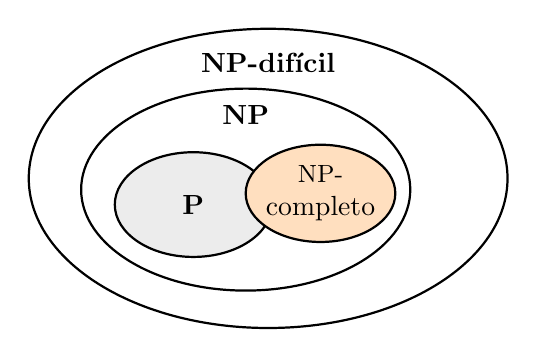
\begin{tikzpicture}[scale=0.95]
        \draw[thick] (0,0) ellipse (3.2 and 2.0);
        \node at (0,1.55) {\textbf{NP-difícil}};
        \draw[thick] (-0.3,-0.15) ellipse (2.2 and 1.35);
        \node at (-0.3,0.85) {\textbf{NP}};
        \draw[thick,fill=gray!15] (-1.0,-0.35) ellipse (1.05 and 0.7);
        \node at (-1.0,-0.35) {\textbf{P}};
        \draw[thick,fill=orange!25] (0.7,-0.2) ellipse (1.0 and 0.65);
        \node[align=center] at (0.7,-0.2) {\small NP-\\completo};
    \end{tikzpicture}
    \caption{Inclusão esquemática das classes (hipótese $P \neq NP$).}
    \fonte{Elaborado pelo autor.}
    \label{fig:inclusao}
\end{figure}

% ============================================================
\chapter{TÉCNICAS DE APROXIMAÇÃO E HEURÍSTICAS}
\label{cap:tecnicas}

Problemas NP-completos raramente admitem solução ótima polinomial (salvo se $P=NP$). Na engenharia, ``otimizar'' um NP-completo costuma significar buscar soluções boas o bastante com técnicas de aproximação ou heurística \cite{cormen,garey}. A seguir, cada técnica do enunciado.

\section{HEURÍSTICA}
\label{sec:heuristica}

Heurística é qualquer regra prática que guia a busca sem garantir ótimo nem, em geral, razão de aproximação. Exemplos: buscar local (trocar dois vértices num tour do TSP se o custo cair), simulated annealing, tabu search. No Independent Set, uma heurística simples é repetidamente pegar o vértice de menor grau e remover seus vizinhos. Vantagens: implementação rápida e bom comportamento médio em instâncias reais. Limite: pode ficar arbitrariamente longe do ótimo e a análise formal é difícil. Em relação a P/NP, a heurística não ``tira'' o problema de NP-difícil; apenas evita enumerar $2^n$ candidatos na prática.

\section{ALGORITMO GULOSO}
\label{sec:guloso}

O guloso constrói a solução escolha a escolha, sempre pegando o passo localmente melhor, sem voltar atrás. No Caixeiro Viajante, o vizinho mais próximo é guloso; na Mochila fracionária, ordenar por valor/peso é ótimo; na Mochila 0/1, o mesmo critério é só aproximação. Cormen \textit{et al.} mostram que a Mochila fracionária cai em P pelo guloso, enquanto a 0/1 permanece NP-difícil na otimização \cite{cormen}. Complexidade típica: $O(n \log n)$ pela ordenação. Em troca da velocidade, perde-se otimalidade --- na Seção~\ref{sec:testes} o guloso erra em instâncias maiores.

\section{PROGRAMAÇÃO LINEAR}
\label{sec:pl}

Programação linear (PL) otimiza função linear sob desigualdades lineares. Em tempo polinomial (elipsoide / métodos de ponto interior) resolve-se a relaxação contínua de vários problemas combinatórios. A estratégia clássica é: escrever a formulação inteira (PLI), relaxar as variáveis $x_i \in \{0,1\}$ para $x_i \in [0,1]$, resolver a PL e arredondar. Para Vertex Cover há $2$-aproximação via relaxação; para Max-Cut e outros, algoritmos de Goemans--Williamson usam SDP (relaxação ainda mais forte). Na Mochila, a relaxação fracionária dá um limitante superior e inspira o guloso por densidade. O ponto-chave para complexidade: a PL está em P; a parte NP-difícil volta quando se exige integralidade.

\section{ALGORITMOS GENÉTICOS}
\label{sec:ag}

Algoritmos genéticos mantêm uma população de soluções candidatas (cromossomos), avaliam aptidão (fitness), selecionam pais, cruzam e mutam. No TSP, um cromossomo é uma permutação de cidades; no Knapsack, um vetor binário de inclusão de itens (reparando peso excedente). São meta-heurísticas estocásticas: não garantem ótimo, mas exploram bem espaços grandes quando a função objetivo é barata de avaliar. Parâmetros (tamanho da população, taxa de mutação, elitismo) afetam muito o resultado. Do ponto de vista teórico, AG não coloca o problema em P; do ponto de vista prático, são úteis quando a instância é grande demais para PD ou branch-and-bound.

\section{PROGRAMAÇÃO DINÂMICA}
\label{sec:pd}

Programação dinâmica (PD) decompõe o problema em subproblemas sobrepostos com estrutura ótima e memoriza respostas. Na Mochila 0/1, $dp[i][w]$ é o melhor valor usando os $i$ primeiros itens e capacidade $w$; a recorrência é
\[
dp[i][w] = \max\bigl(dp[i-1][w],\; dp[i-1][w-p_i] + v_i\bigr)
\]
quando $p_i \leq w$. Tempo e memória $O(nW)$ --- \textit{pseudo-polinomial}: polinomial em $n$ e no valor numérico $W$, não no número de bits de $W$. Por isso a decisão da Mochila continua NP-completa (quando $W$ é exponencial no tamanho da entrada) mesmo existindo PD ``rápida'' para $W$ moderado \cite{garey,cormen}. PD também resolve caminho mais longo em DAGs, distância de edição e vários problemas em P; em grafos gerais, Longest Path permanece NP-completo.

\begin{quadro}[!h]
    \centering
    \legenda[quad:tecnicas]{SÍNTESE DAS TÉCNICAS}
    \small
    \begin{tabular}{|p{2.8cm}|p{4.0cm}|p{5.4cm}|}
        \hline
        \textbf{Técnica} & \textbf{Garantia} & \textbf{Uso típico} \\
        \hline
        Heurística & nenhuma & busca local, regras de domínio \\
        \hline
        Guloso & às vezes razão fixa & Mochila fracionária; coberturas \\
        \hline
        PL / relaxação & bound + arredondamento & Vertex Cover, Max-Cut \\
        \hline
        Genéticos & nenhuma (estocástico) & TSP e Knapsack grandes \\
        \hline
        PD & ótimo se couber em $W$ & Mochila 0/1 com $W$ moderado \\
        \hline
    \end{tabular}
    \fonte{Elaborado pelo autor.}
\end{quadro}

% ============================================================
\chapter{PARTE PRÁTICA --- PROBLEMA DA MOCHILA}
\label{cap:pratica}

\section{DESCRIÇÃO DO PROBLEMA}
\label{sec:desc}

Dado um conjunto de $n$ itens, cada um com peso $p_i$ e valor $v_i$, e uma capacidade $W$, a \textbf{Mochila 0/1} pede um subconjunto $S$ que maximize $\sum_{i \in S} v_i$ sujeito a $\sum_{i \in S} p_i \leq W$. A versão de decisão (existe $S$ com valor $\geq V$ e peso $\leq W$?) é NP-completa \cite{garey,karp}. Escolhemos este problema por três motivos: (i) aparece na lista do enunciado; (ii) o contraste entre força bruta e PD é didático; (iii) o guloso por densidade ilustra heurística sem garantia.

\section{ALGORITMO BURRO (FORÇA BRUTA)}
\label{sec:burro}

O algoritmo burro enumera os $2^n$ subconjuntos (máscaras de bits), descarta os que excedem $W$ e guarda o de maior valor. Pseudocódigo:

\begin{lstlisting}[language=Python]
melhor = 0
for mascara in range(1 << n):
    peso = valor = 0
    for i in range(n):
        if mascara & (1 << i):
            peso += p[i]; valor += v[i]
            if peso > W: break
    if peso <= W and valor > melhor:
        melhor = valor
\end{lstlisting}

Complexidade de tempo $O(2^n \cdot n)$ e memória $O(1)$ além da entrada. Correto, mas inviável para $n > 30$.

\section{ALGORITMO EXATO VIA PROGRAMAÇÃO DINÂMICA}
\label{sec:exato}

A PD da Seção~\ref{sec:pd} preenche uma tabela $(n+1)\times(W+1)$ e reconstrói os itens escolhidos. Tempo $O(nW)$, memória $O(nW)$ (otimizável para $O(W)$ se só o valor ótimo for necessário). Continua sendo um algoritmo para um problema NP-completo: a ``armadilha'' está em $W$ poder ser exponencial na entrada.

\section{ANÁLISE DE EFICIÊNCIA}
\label{sec:eficiencia}

\begin{quadro}[!h]
    \centering
    \legenda[quad:complex]{COMPLEXIDADE ASSINTÓTICA}
    \small
    \begin{tabular}{|l|l|l|}
        \hline
        \textbf{Algoritmo} & \textbf{Tempo} & \textbf{Espaço} \\
        \hline
        Força bruta & $O(2^n \cdot n)$ & $O(1)$ \\
        \hline
        Programação dinâmica & $O(nW)$ & $O(nW)$ \\
        \hline
        Guloso por densidade & $O(n \log n)$ & $O(n)$ \\
        \hline
    \end{tabular}
    \fonte{Elaborado pelo autor.}
\end{quadro}

A Figura~\ref{fig:tempos} mostra tempos medidos em Python 3.12 nesta máquina. A força bruta explode perto de $n=18$ ($\approx 155$\,ms), enquanto a PD permanece abaixo de $0{,}1$\,ms com $W$ da ordem de dezenas.

\begin{figure}[!h]
    \centering
    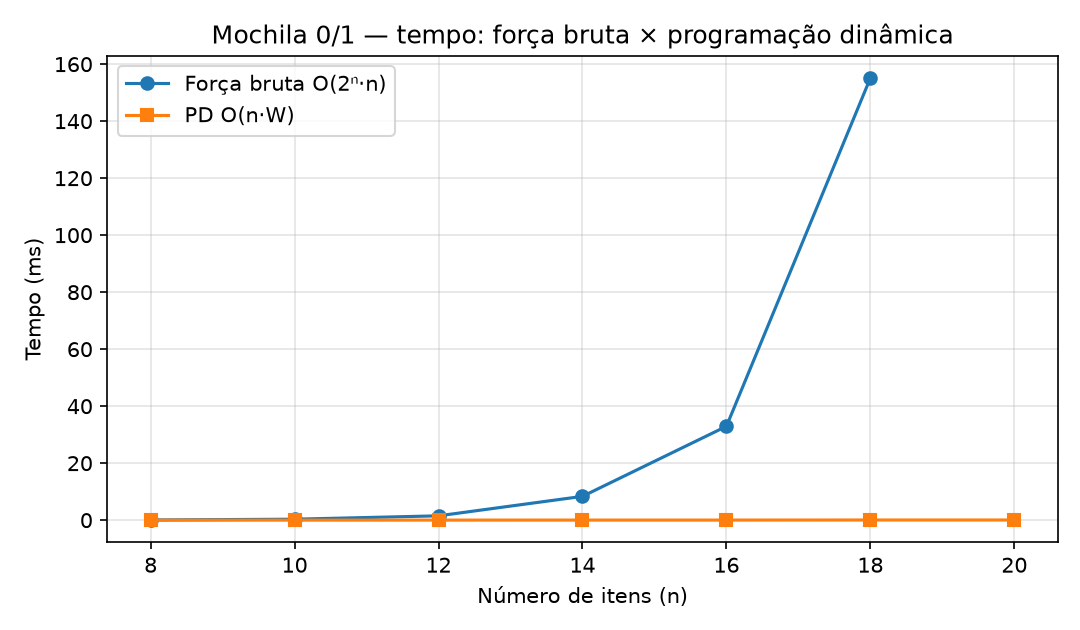
\includegraphics[width=0.92\textwidth]{mochila-tempos.png}
    \caption{Tempo de execução: força bruta versus PD em função de $n$.}
    \fonte{Elaborado pelo autor (script \texttt{ed2-mochila.py}).}
    \label{fig:tempos}
\end{figure}

\section{PROGRAMAÇÃO E TESTES}
\label{sec:testes}

O programa \texttt{material/exercicios/ed2-mochila.py} implementa os três algoritmos, imprime resultados e pode gerar o gráfico com \texttt{--grafico}. Na instância didática ($n=5$, $W=8$), FB e PD concordam no ótimo $13$ (itens caderno, livro, fone); o guloso também acerta nesse caso. Em $n=22$, a PD obtém valor $274$ e o guloso $272$, evidenciando a perda de otimalidade. A Figura~\ref{fig:tela} reproduz a saída do terminal.

\begin{figure}[!h]
    \centering
    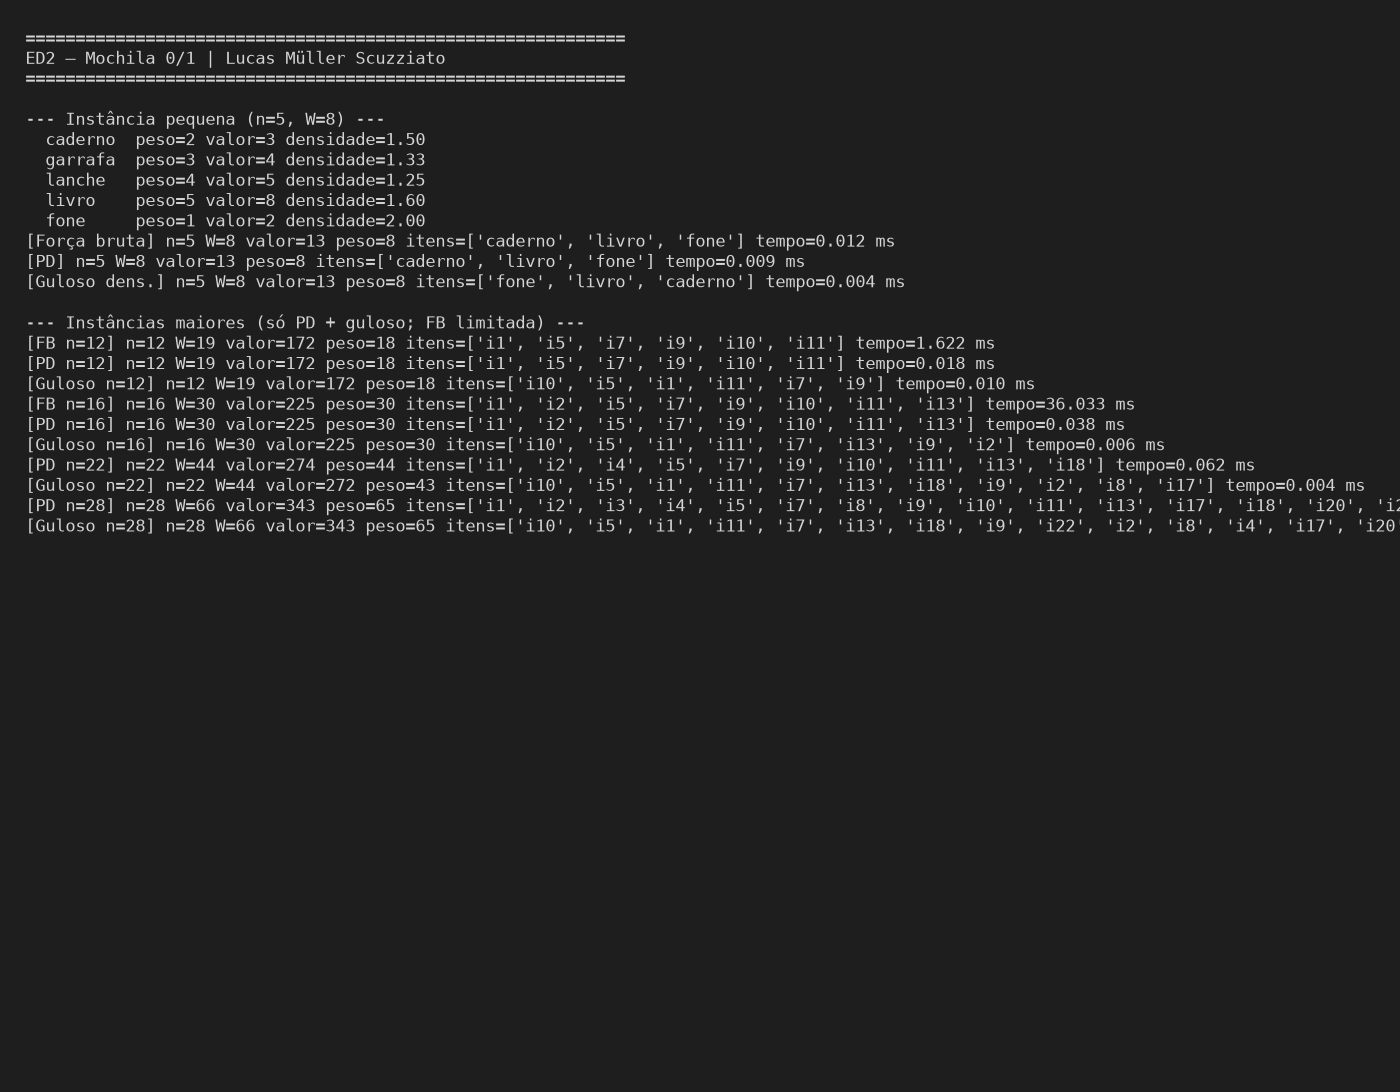
\includegraphics[width=0.95\textwidth]{tela-testes.png}
    \caption{Tela de execução dos testes (instância pequena e instâncias maiores).}
    \fonte{Elaborado pelo autor.}
    \label{fig:tela}
\end{figure}

Trecho essencial da PD:

\begin{lstlisting}[language=Python]
# Autor: Lucas Müller Scuzziato
def programacao_dinamica(itens, capacidade):
    n = len(itens)
    dp = [[0] * (capacidade + 1) for _ in range(n + 1)]
    for i in range(1, n + 1):
        _, peso, valor = itens[i - 1]
        for w in range(capacidade + 1):
            dp[i][w] = dp[i - 1][w]
            if peso <= w:
                candidato = dp[i - 1][w - peso] + valor
                if candidato > dp[i][w]:
                    dp[i][w] = candidato
    # ... reconstrução dos itens omitida ...
    return dp[n][capacidade]
\end{lstlisting}

Como validar: \texttt{python3 material/exercicios/ed2-mochila.py}. Os valores de FB e PD devem coincidir sempre que ambos rodarem; o guloso pode divergir.

\apendices

\chapter{CÓDIGO-FONTE COMPLETO}
\label{ap:codigo}

O arquivo-fonte completo (com o nome do autor em comentário, conforme o enunciado) é \texttt{ed2-mochila.py}. Para regenerar os testes e o gráfico:

\begin{lstlisting}[language=bash]
python3 ed2-mochila.py --grafico mochila-tempos.png
\end{lstlisting}

O programa implementa força bruta, programação dinâmica e guloso por densidade; imprime tempos e soluções; e, com \texttt{--grafico}, grava a Figura~\ref{fig:tempos}.

\postextual
\bibliography{referencias}

\end{document}
